\documentclass[ignorenonframetext,]{beamer}
\setbeamertemplate{caption}[numbered]
\setbeamertemplate{caption label separator}{: }
\setbeamercolor{caption name}{fg=normal text.fg}
\beamertemplatenavigationsymbolsempty
\usepackage{lmodern}
\usepackage{amssymb,amsmath}
\usepackage{ifxetex,ifluatex}
\usepackage{fixltx2e} % provides \textsubscript
\ifnum 0\ifxetex 1\fi\ifluatex 1\fi=0 % if pdftex
  \usepackage[T1]{fontenc}
  \usepackage[utf8]{inputenc}
\else % if luatex or xelatex
  \ifxetex
    \usepackage{mathspec}
  \else
    \usepackage{fontspec}
  \fi
  \defaultfontfeatures{Ligatures=TeX,Scale=MatchLowercase}
\fi
\usetheme[]{Warsaw}
\usefonttheme{structurebold}
% use upquote if available, for straight quotes in verbatim environments
\IfFileExists{upquote.sty}{\usepackage{upquote}}{}
% use microtype if available
\IfFileExists{microtype.sty}{%
\usepackage{microtype}
\UseMicrotypeSet[protrusion]{basicmath} % disable protrusion for tt fonts
}{}
\newif\ifbibliography
\hypersetup{
            pdftitle={Características Básicas de R},
            pdfauthor={Santiago Lozano},
            pdfborder={0 0 0},
            breaklinks=true}
\urlstyle{same}  % don't use monospace font for urls
\usepackage{color}
\usepackage{fancyvrb}
\newcommand{\VerbBar}{|}
\newcommand{\VERB}{\Verb[commandchars=\\\{\}]}
\DefineVerbatimEnvironment{Highlighting}{Verbatim}{commandchars=\\\{\}}
% Add ',fontsize=\small' for more characters per line
\usepackage{framed}
\definecolor{shadecolor}{RGB}{248,248,248}
\newenvironment{Shaded}{\begin{snugshade}}{\end{snugshade}}
\newcommand{\KeywordTok}[1]{\textcolor[rgb]{0.13,0.29,0.53}{\textbf{#1}}}
\newcommand{\DataTypeTok}[1]{\textcolor[rgb]{0.13,0.29,0.53}{#1}}
\newcommand{\DecValTok}[1]{\textcolor[rgb]{0.00,0.00,0.81}{#1}}
\newcommand{\BaseNTok}[1]{\textcolor[rgb]{0.00,0.00,0.81}{#1}}
\newcommand{\FloatTok}[1]{\textcolor[rgb]{0.00,0.00,0.81}{#1}}
\newcommand{\ConstantTok}[1]{\textcolor[rgb]{0.00,0.00,0.00}{#1}}
\newcommand{\CharTok}[1]{\textcolor[rgb]{0.31,0.60,0.02}{#1}}
\newcommand{\SpecialCharTok}[1]{\textcolor[rgb]{0.00,0.00,0.00}{#1}}
\newcommand{\StringTok}[1]{\textcolor[rgb]{0.31,0.60,0.02}{#1}}
\newcommand{\VerbatimStringTok}[1]{\textcolor[rgb]{0.31,0.60,0.02}{#1}}
\newcommand{\SpecialStringTok}[1]{\textcolor[rgb]{0.31,0.60,0.02}{#1}}
\newcommand{\ImportTok}[1]{#1}
\newcommand{\CommentTok}[1]{\textcolor[rgb]{0.56,0.35,0.01}{\textit{#1}}}
\newcommand{\DocumentationTok}[1]{\textcolor[rgb]{0.56,0.35,0.01}{\textbf{\textit{#1}}}}
\newcommand{\AnnotationTok}[1]{\textcolor[rgb]{0.56,0.35,0.01}{\textbf{\textit{#1}}}}
\newcommand{\CommentVarTok}[1]{\textcolor[rgb]{0.56,0.35,0.01}{\textbf{\textit{#1}}}}
\newcommand{\OtherTok}[1]{\textcolor[rgb]{0.56,0.35,0.01}{#1}}
\newcommand{\FunctionTok}[1]{\textcolor[rgb]{0.00,0.00,0.00}{#1}}
\newcommand{\VariableTok}[1]{\textcolor[rgb]{0.00,0.00,0.00}{#1}}
\newcommand{\ControlFlowTok}[1]{\textcolor[rgb]{0.13,0.29,0.53}{\textbf{#1}}}
\newcommand{\OperatorTok}[1]{\textcolor[rgb]{0.81,0.36,0.00}{\textbf{#1}}}
\newcommand{\BuiltInTok}[1]{#1}
\newcommand{\ExtensionTok}[1]{#1}
\newcommand{\PreprocessorTok}[1]{\textcolor[rgb]{0.56,0.35,0.01}{\textit{#1}}}
\newcommand{\AttributeTok}[1]{\textcolor[rgb]{0.77,0.63,0.00}{#1}}
\newcommand{\RegionMarkerTok}[1]{#1}
\newcommand{\InformationTok}[1]{\textcolor[rgb]{0.56,0.35,0.01}{\textbf{\textit{#1}}}}
\newcommand{\WarningTok}[1]{\textcolor[rgb]{0.56,0.35,0.01}{\textbf{\textit{#1}}}}
\newcommand{\AlertTok}[1]{\textcolor[rgb]{0.94,0.16,0.16}{#1}}
\newcommand{\ErrorTok}[1]{\textcolor[rgb]{0.64,0.00,0.00}{\textbf{#1}}}
\newcommand{\NormalTok}[1]{#1}

% Prevent slide breaks in the middle of a paragraph:
\widowpenalties 1 10000
\raggedbottom

\AtBeginPart{
  \let\insertpartnumber\relax
  \let\partname\relax
  \frame{\partpage}
}
\AtBeginSection{
  \ifbibliography
  \else
    \let\insertsectionnumber\relax
    \let\sectionname\relax
    \frame{\sectionpage}
  \fi
}
\AtBeginSubsection{
  \let\insertsubsectionnumber\relax
  \let\subsectionname\relax
  \frame{\subsectionpage}
}

\setlength{\parindent}{0pt}
\setlength{\parskip}{6pt plus 2pt minus 1pt}
\setlength{\emergencystretch}{3em}  % prevent overfull lines
\providecommand{\tightlist}{%
  \setlength{\itemsep}{0pt}\setlength{\parskip}{0pt}}
\setcounter{secnumdepth}{0}

\title{Características Básicas de R}
\author{Santiago Lozano}
\date{27 de enero de 2020}

\begin{document}
\frame{\titlepage}

\begin{frame}[fragile]{Calculadora}

Como otros lenguajes similares, R puede facilmente reemplzar todas las
funcionalidades de una calculadora y de manera más eficiente, una de sus
mayores fortalezas es que R permite las operaciones entre arreglos
(arrays)

\begin{Shaded}
\begin{Highlighting}[]
\DecValTok{5} \OperatorTok{+}\StringTok{ }\DecValTok{7}
\end{Highlighting}
\end{Shaded}

\begin{verbatim}
## [1] 12
\end{verbatim}

\end{frame}

\begin{frame}[fragile]{Calculadora}

\begin{Shaded}
\begin{Highlighting}[]
\KeywordTok{log}\NormalTok{(}\DecValTok{42}\OperatorTok{/}\FloatTok{7.3}\NormalTok{)}
\end{Highlighting}
\end{Shaded}

\begin{verbatim}
## [1] 1.749795
\end{verbatim}

Cada línea puede tener a lo sumo 8192 carateres, pero si se quiere tener
una instrucción o una expresión en la pantalla visualmente más legible,
se puede continuar en las líneas de abajo simplemente cambiando la línea

\begin{Shaded}
\begin{Highlighting}[]
\DecValTok{5} \OperatorTok{+}\StringTok{ }\DecValTok{6} \OperatorTok{+}\StringTok{ }\DecValTok{3} \OperatorTok{+}\StringTok{ }\DecValTok{6} \OperatorTok{+}\StringTok{ }\DecValTok{4} \OperatorTok{+}\StringTok{ }\DecValTok{2} \OperatorTok{+}\StringTok{ }\DecValTok{4} \OperatorTok{+}\StringTok{ }\DecValTok{8} \OperatorTok{+}
\StringTok{  }\DecValTok{3} \OperatorTok{+}\StringTok{ }\DecValTok{2} \OperatorTok{+}\StringTok{ }\DecValTok{7}
\end{Highlighting}
\end{Shaded}

\begin{verbatim}
## [1] 50
\end{verbatim}

\end{frame}

\begin{frame}[fragile]{Calculadora}

también se puede usar punto y coma (;) para separar varias instrucciones

\begin{Shaded}
\begin{Highlighting}[]
\DecValTok{2} \OperatorTok{+}\StringTok{ }\DecValTok{3}\NormalTok{; }\DecValTok{5} \OperatorTok{*}\StringTok{ }\DecValTok{7}\NormalTok{; }\DecValTok{3} \OperatorTok{-}\StringTok{ }\DecValTok{7}
\end{Highlighting}
\end{Shaded}

\begin{verbatim}
## [1] 5
\end{verbatim}

\begin{verbatim}
## [1] 35
\end{verbatim}

\begin{verbatim}
## [1] -4
\end{verbatim}

\end{frame}

\begin{frame}[fragile]{Calculadora}

y los grandes números pueden ser expuestos en notación científica

\begin{Shaded}
\begin{Highlighting}[]
\FloatTok{1.2e3} \CommentTok{#1200}
\end{Highlighting}
\end{Shaded}

\begin{verbatim}
## [1] 1200
\end{verbatim}

\begin{Shaded}
\begin{Highlighting}[]
\FloatTok{1.2e-2} \CommentTok{#0.012}
\end{Highlighting}
\end{Shaded}

\begin{verbatim}
## [1] 0.012
\end{verbatim}

a su vez, es posible relizar operaciones entre arreglos

\begin{Shaded}
\begin{Highlighting}[]
\KeywordTok{c}\NormalTok{(}\DecValTok{1}\NormalTok{, }\DecValTok{2}\NormalTok{, }\DecValTok{3}\NormalTok{, }\DecValTok{4}\NormalTok{, }\DecValTok{5}\NormalTok{) }\OperatorTok{*}\StringTok{ }\DecValTok{2}
\end{Highlighting}
\end{Shaded}

\begin{verbatim}
## [1]  2  4  6  8 10
\end{verbatim}

\end{frame}

\begin{frame}[fragile]{Calculadora}

Los símbolos aritméticos corresponden a + (suma), - (resta), *
(multiplicación), / (división), \%\% (módulo: Residuo de la división),
\%\% (cociente de la división)

\begin{Shaded}
\begin{Highlighting}[]
\DecValTok{119} \OperatorTok\StringTok{ }\DecValTok{13}
\end{Highlighting}
\end{Shaded}

\begin{verbatim}
## [1] 9
\end{verbatim}

\begin{Shaded}
\begin{Highlighting}[]
\DecValTok{119} \OperatorTok\StringTok{ }\DecValTok{13}
\end{Highlighting}
\end{Shaded}

\begin{verbatim}
## [1] 2
\end{verbatim}

\end{frame}

\begin{frame}[fragile]{Calculadora}

\begin{Shaded}
\begin{Highlighting}[]
\DecValTok{9} \OperatorTok\StringTok{ }\DecValTok{2}
\end{Highlighting}
\end{Shaded}

\begin{verbatim}
## [1] 1
\end{verbatim}

\begin{Shaded}
\begin{Highlighting}[]
\DecValTok{8} \OperatorTok\StringTok{ }\DecValTok{2}
\end{Highlighting}
\end{Shaded}

\begin{verbatim}
## [1] 0
\end{verbatim}

\end{frame}

\begin{frame}[fragile]{Calculadora}

\textbf{PEMDAS}

\begin{itemize}
\tightlist
\item
  Paréntesis
\item
  Exponenciales
\item
  Multiplicación
\item
  División
\item
  Adición
\item
  Sustracción
\end{itemize}

\begin{Shaded}
\begin{Highlighting}[]
\DecValTok{6}\OperatorTok{/}\DecValTok{3}\OperatorTok{+}\DecValTok{4}\OperatorTok{*}\DecValTok{2}
\end{Highlighting}
\end{Shaded}

\pause
\begin{verbatim}
## [1] 10
\end{verbatim}

\begin{Shaded}
\begin{Highlighting}[]
\DecValTok{6}\OperatorTok{*}\DecValTok{4}\OperatorTok{-}\DecValTok{12}\OperatorTok{/}\DecValTok{3}\OperatorTok{-}\DecValTok{8}
\end{Highlighting}
\end{Shaded}

\pause
\begin{verbatim}
## [1] 12
\end{verbatim}

\end{frame}

\begin{frame}[fragile]{Calculadora}

\begin{Shaded}
\begin{Highlighting}[]
\DecValTok{4}\OperatorTok{*}\DecValTok{4}\OperatorTok{-}\DecValTok{3}\OperatorTok{*}\DecValTok{3}\OperatorTok{-}\DecValTok{16}\OperatorTok{/}\DecValTok{4}
\end{Highlighting}
\end{Shaded}

\pause
\begin{verbatim}
## [1] 3
\end{verbatim}

\begin{Shaded}
\begin{Highlighting}[]
\DecValTok{20}\OperatorTok{-}\NormalTok{(}\DecValTok{3}\OperatorTok{*}\DecValTok{2}\OperatorTok{^}\DecValTok{3}\OperatorTok{-}\DecValTok{5}\NormalTok{)}
\end{Highlighting}
\end{Shaded}

\pause
\begin{verbatim}
## [1] 1
\end{verbatim}

\begin{Shaded}
\begin{Highlighting}[]
\NormalTok{(}\DecValTok{5}\OperatorTok{+}\DecValTok{2}\NormalTok{)}\OperatorTok{^}\DecValTok{2}\OperatorTok{-}\DecValTok{9}\OperatorTok{*}\DecValTok{3}\OperatorTok{+}\DecValTok{2}\OperatorTok{^}\DecValTok{3}
\end{Highlighting}
\end{Shaded}

\pause
\begin{verbatim}
## [1] 30
\end{verbatim}

\end{frame}

\begin{frame}[fragile]{Calculadora}

\begin{Shaded}
\begin{Highlighting}[]
\NormalTok{(}\DecValTok{2}\OperatorTok{^}\DecValTok{4}\OperatorTok{+}\NormalTok{(}\DecValTok{16}\OperatorTok{-}\DecValTok{3}\OperatorTok{*}\DecValTok{4}\NormalTok{))}\OperatorTok{/}\NormalTok{((}\DecValTok{6}\OperatorTok{+}\DecValTok{3}\OperatorTok{^}\DecValTok{2}\NormalTok{)}\OperatorTok{/}\NormalTok{(}\DecValTok{7}\OperatorTok{-}\DecValTok{4}\NormalTok{))}
\end{Highlighting}
\end{Shaded}

\pause
\begin{verbatim}
## [1] 4
\end{verbatim}

\end{frame}

\begin{frame}[fragile]{Redondeo}

Tenemos varios tipos de Redondeo

\begin{itemize}
\tightlist
\item
  \textbf{El entero más grande menor que}
\end{itemize}

\begin{Shaded}
\begin{Highlighting}[]
\KeywordTok{floor}\NormalTok{(}\FloatTok{5.7}\NormalTok{)}
\end{Highlighting}
\end{Shaded}

\begin{verbatim}
## [1] 5
\end{verbatim}

\begin{itemize}
\tightlist
\item
  \textbf{El entero siguiente}
\end{itemize}

\begin{Shaded}
\begin{Highlighting}[]
\KeywordTok{ceiling}\NormalTok{(}\FloatTok{5.7}\NormalTok{)}
\end{Highlighting}
\end{Shaded}

\begin{verbatim}
## [1] 6
\end{verbatim}

\end{frame}

\begin{frame}[fragile]{Redondeo}

\begin{itemize}
\tightlist
\item
  \textbf{Lugar decimal}: Especificando bajo que lugar decimal se hace
  la aproximación
\end{itemize}

\begin{Shaded}
\begin{Highlighting}[]
\KeywordTok{round}\NormalTok{(}\FloatTok{5.7}\NormalTok{,}\DecValTok{0}\NormalTok{)}
\end{Highlighting}
\end{Shaded}

\begin{verbatim}
## [1] 6
\end{verbatim}

\end{frame}

\begin{frame}[fragile]{Redondeo}

\begin{Shaded}
\begin{Highlighting}[]
\KeywordTok{round}\NormalTok{(}\FloatTok{5.4}\NormalTok{,}\DecValTok{0}\NormalTok{)}
\end{Highlighting}
\end{Shaded}

\begin{verbatim}
## [1] 5
\end{verbatim}

\begin{Shaded}
\begin{Highlighting}[]
\NormalTok{x2 <-}\StringTok{ }\NormalTok{pi }\OperatorTok{*}\StringTok{ }\DecValTok{100}\OperatorTok{^}\NormalTok{(}\OperatorTok{-}\DecValTok{1}\OperatorTok{:}\DecValTok{3}\NormalTok{)}
\NormalTok{x2}
\end{Highlighting}
\end{Shaded}

\begin{verbatim}
## [1] 3.141593e-02 3.141593e+00 3.141593e+02 
## [4] 3.141593e+04 3.141593e+06
\end{verbatim}

\begin{Shaded}
\begin{Highlighting}[]
\KeywordTok{round}\NormalTok{(x2, }\DecValTok{3}\NormalTok{)}
\end{Highlighting}
\end{Shaded}

\begin{verbatim}
## [1]  0.031  3.142  314.159 31415.927 3141592.654
\end{verbatim}

\end{frame}

\begin{frame}[fragile]{Redondeo}

\begin{itemize}
\tightlist
\item
  \textbf{Dígitos de Significancia}
\end{itemize}

\begin{Shaded}
\begin{Highlighting}[]
\KeywordTok{signif}\NormalTok{(}\DecValTok{12345678}\NormalTok{,}\DecValTok{4}\NormalTok{)}
\end{Highlighting}
\end{Shaded}

\begin{verbatim}
## [1] 12350000
\end{verbatim}

\begin{Shaded}
\begin{Highlighting}[]
\KeywordTok{signif}\NormalTok{(}\DecValTok{12345678}\NormalTok{,}\DecValTok{5}\NormalTok{)}
\end{Highlighting}
\end{Shaded}

\begin{verbatim}
## [1] 12346000
\end{verbatim}

\begin{Shaded}
\begin{Highlighting}[]
\KeywordTok{signif}\NormalTok{(}\DecValTok{12345678}\NormalTok{,}\DecValTok{3}\NormalTok{)}
\end{Highlighting}
\end{Shaded}

\begin{verbatim}
## [1] 12300000
\end{verbatim}

\end{frame}

\begin{frame}{Funciones Matemáticas}

\begin{center}
\begin{figure}
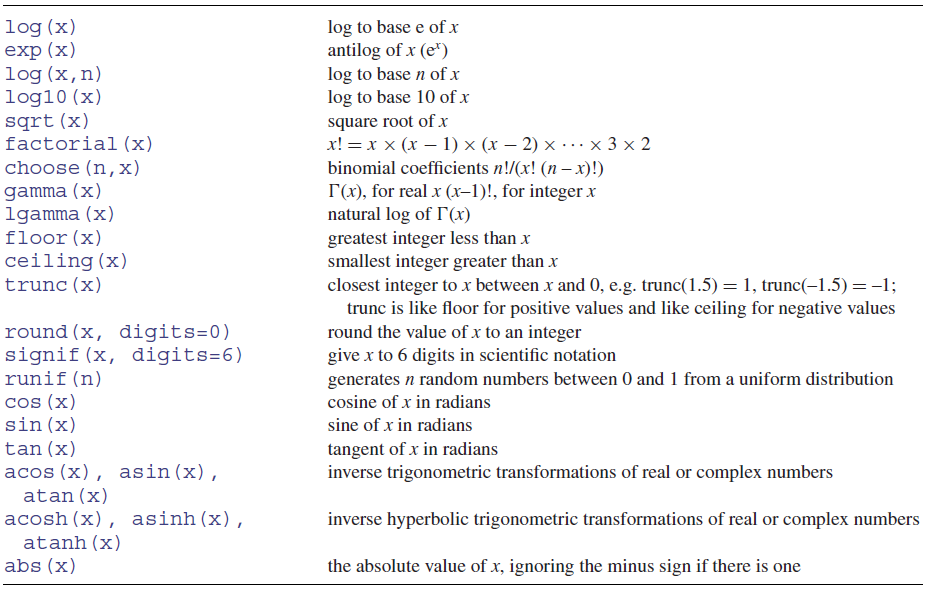
\includegraphics[scale=0.4]{funciones.png}
\end{figure}
\end{center}

\end{frame}

\begin{frame}[fragile]{Asignación de Variables}

En los campos anteriores observábamos que los resultados se obtenían
directamente en la ventana de comandos, sin embargo, R es un lenguaje de
progrmación y a menudo la razón de usar un lenguaje de programación como
opuesto a una calculadora es automatizar algún proceso o establecer
repeticiones.

Por ejemplo, quisierámos usar el resultado de 5 + 7 en un segundo
cálculo y en vez de repetir aquella sentencia podemos crear una variable
que la almacene mediante \textless{}- una flecha hacía la izquierda

\begin{Shaded}
\begin{Highlighting}[]
\NormalTok{x <-}\StringTok{ }\DecValTok{5} \OperatorTok{+}\StringTok{ }\DecValTok{7}
\end{Highlighting}
\end{Shaded}

para ver el contenido de la variable x, simplemente la escribimos

\begin{Shaded}
\begin{Highlighting}[]
\NormalTok{x}
\end{Highlighting}
\end{Shaded}

\begin{verbatim}
## [1] 12
\end{verbatim}

\end{frame}

\begin{frame}[fragile]{Asignación de Variables}

Es erróneo tipear

\begin{Shaded}
\begin{Highlighting}[]
\NormalTok{x }\OperatorTok{<}\StringTok{ }\OperatorTok{-}\StringTok{ }\DecValTok{5} \OperatorTok{+}\StringTok{ }\DecValTok{7}
\end{Highlighting}
\end{Shaded}

\begin{verbatim}
## [1] FALSE
\end{verbatim}

Ahora

\begin{Shaded}
\begin{Highlighting}[]
\NormalTok{y <-}\StringTok{ }\NormalTok{x }\OperatorTok{-}\StringTok{ }\DecValTok{3}
\end{Highlighting}
\end{Shaded}

\begin{Shaded}
\begin{Highlighting}[]
\NormalTok{y}
\end{Highlighting}
\end{Shaded}

\begin{verbatim}
## [1] 9
\end{verbatim}

\end{frame}

\begin{frame}{Asignación de Variables}

Algunas cuestiones importante a la hora de establecer variables

\begin{itemize}
\item
  Cuando a algún valor no le asignamos alguna variable este no se
  almacena, pero si le asignamos una variable, esta variable se almacena
  en la memoria RAM, así que es de vital importancia tener un manejo
  debido de esta y evitar tener variables que contengan el mismo valor
\item
  no es lo mismo y que Y
\item
  no se puede poder un nombre de variable con número primero ``1x'' está
  mal, ``x1'' está bien.
\item
  los nombre de las variable no pueden contener espacios
\item
  Evitar poner nombres engorrosos a las variables
\end{itemize}

\end{frame}

\begin{frame}[fragile]{Tipos de Datos en R: Números reales (double)}

\begin{Shaded}
\begin{Highlighting}[]
\NormalTok{a <-}\StringTok{ }\DecValTok{1}
\NormalTok{b <-}\StringTok{ }\FloatTok{3.4}
\NormalTok{c <-}\StringTok{ }\NormalTok{pi}
\end{Highlighting}
\end{Shaded}

\begin{Shaded}
\begin{Highlighting}[]
\KeywordTok{is.double}\NormalTok{(a)}
\end{Highlighting}
\end{Shaded}

\begin{verbatim}
## [1] TRUE
\end{verbatim}

\end{frame}

\begin{frame}[fragile]{Tipos de datos en R: Números reales (double)}

\begin{Shaded}
\begin{Highlighting}[]
\KeywordTok{is.double}\NormalTok{(b)}
\end{Highlighting}
\end{Shaded}

\begin{verbatim}
## [1] TRUE
\end{verbatim}

\begin{Shaded}
\begin{Highlighting}[]
\KeywordTok{is.double}\NormalTok{(c)}
\end{Highlighting}
\end{Shaded}

\begin{verbatim}
## [1] TRUE
\end{verbatim}

\begin{Shaded}
\begin{Highlighting}[]
\KeywordTok{typeof}\NormalTok{(b)}
\end{Highlighting}
\end{Shaded}

\begin{verbatim}
## [1] "double"
\end{verbatim}

\end{frame}

\begin{frame}[fragile]{Tipos de datos en R: Número entero (integer)}

Inicialmente los número son enteros y reales a la misma vez son
establecidos como double, pero estos pueden ser transformados a integer,
otra nota importante que puede ser tenida en cuenta es que los integer
consumen menos memoria que los numeric

\begin{Shaded}
\begin{Highlighting}[]
\NormalTok{d <-}\StringTok{ }\KeywordTok{as.integer}\NormalTok{(a)}
\end{Highlighting}
\end{Shaded}

\begin{Shaded}
\begin{Highlighting}[]
\KeywordTok{is.integer}\NormalTok{(d)}
\end{Highlighting}
\end{Shaded}

\begin{verbatim}
## [1] TRUE
\end{verbatim}

\begin{Shaded}
\begin{Highlighting}[]
\KeywordTok{typeof}\NormalTok{(d)}
\end{Highlighting}
\end{Shaded}

\begin{verbatim}
## [1] "integer"
\end{verbatim}

\end{frame}

\begin{frame}[fragile]{Tipos de datos en R: Números complejos (complex)}

Los números complejos pueden ser creados gracias a la letra i

\begin{Shaded}
\begin{Highlighting}[]
\NormalTok{1i}
\end{Highlighting}
\end{Shaded}

\begin{verbatim}
## [1] 0+1i
\end{verbatim}

\begin{Shaded}
\begin{Highlighting}[]
\NormalTok{z <-}\StringTok{ }\DecValTok{1} \OperatorTok{+}\StringTok{ }\NormalTok{2i}
\end{Highlighting}
\end{Shaded}

\begin{Shaded}
\begin{Highlighting}[]
\KeywordTok{typeof}\NormalTok{(z)}
\end{Highlighting}
\end{Shaded}

\begin{verbatim}
## [1] "complex"
\end{verbatim}

\end{frame}

\begin{frame}[fragile]{Tipos de datos en R: Números complejos (complex)}

\begin{Shaded}
\begin{Highlighting}[]
\KeywordTok{is.complex}\NormalTok{(z)}
\end{Highlighting}
\end{Shaded}

\begin{verbatim}
## [1] TRUE
\end{verbatim}

\begin{Shaded}
\begin{Highlighting}[]
\KeywordTok{Re}\NormalTok{(z)}
\end{Highlighting}
\end{Shaded}

\begin{verbatim}
## [1] 1
\end{verbatim}

\begin{Shaded}
\begin{Highlighting}[]
\KeywordTok{Im}\NormalTok{(z)}
\end{Highlighting}
\end{Shaded}

\begin{verbatim}
## [1] 2
\end{verbatim}

\end{frame}

\begin{frame}[fragile]{Tipos de datos en R: Números complejos (complex)}

\begin{Shaded}
\begin{Highlighting}[]
\KeywordTok{Mod}\NormalTok{(z)}
\end{Highlighting}
\end{Shaded}

\begin{verbatim}
## [1] 2.236068
\end{verbatim}

\begin{Shaded}
\begin{Highlighting}[]
\KeywordTok{Arg}\NormalTok{(z)}
\end{Highlighting}
\end{Shaded}

\begin{verbatim}
## [1] 1.107149
\end{verbatim}

\end{frame}

\begin{frame}{Tipos de datos en R: Números complejos (complex)}

\begin{center}
\begin{figure}
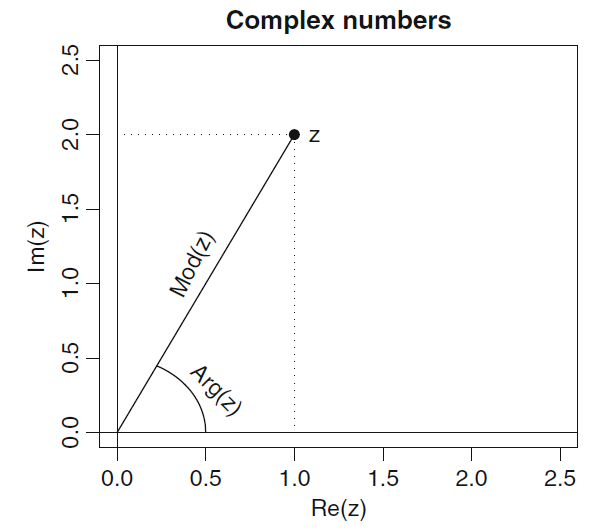
\includegraphics[scale=0.5]{complex.png}
\end{figure}
\end{center}


\end{frame}

\begin{frame}[fragile]{Booleano o de tipo Lógico (logical)}

El tipo logical() es el resultado de una operación lógica. Este puede
tomar los valores TRUE o FALSE, el cálculo de operaciones lógica
corresponde a preguntas sobre cosas

\begin{Shaded}
\begin{Highlighting}[]
\OtherTok{TRUE} \OperatorTok{==}\StringTok{ }\OtherTok{FALSE}
\end{Highlighting}
\end{Shaded}

\begin{verbatim}
## [1] FALSE
\end{verbatim}

\begin{Shaded}
\begin{Highlighting}[]
\NormalTok{T }\OperatorTok{==}\StringTok{ }\NormalTok{F}
\end{Highlighting}
\end{Shaded}

\begin{verbatim}
## [1] FALSE
\end{verbatim}

\end{frame}

\begin{frame}[fragile]{Booleano o de tipo Lógico (logical)}

\begin{Shaded}
\begin{Highlighting}[]
\NormalTok{T <-}\StringTok{ }\DecValTok{0}
\NormalTok{T }\OperatorTok{==}\StringTok{ }\OtherTok{FALSE}
\end{Highlighting}
\end{Shaded}

\begin{verbatim}
## [1] TRUE
\end{verbatim}

\begin{Shaded}
\begin{Highlighting}[]
\NormalTok{F <-}\StringTok{ }\DecValTok{1}
\OtherTok{TRUE} \OperatorTok{==}\StringTok{ }\NormalTok{F}
\end{Highlighting}
\end{Shaded}

\begin{verbatim}
## [1] TRUE
\end{verbatim}

\begin{Shaded}
\begin{Highlighting}[]
\NormalTok{T }\OperatorTok{!=}\StringTok{ }\NormalTok{F}
\end{Highlighting}
\end{Shaded}

\begin{verbatim}
## [1] TRUE
\end{verbatim}

\end{frame}

\begin{frame}[fragile]{Booleano o de tipo Lógico (logical)}

Se debe tener cuidado con los números que contienen dígitos bastante
grandes, pues pueden conducir a diferentes errores pues la mayoría de
números se redondean sobre 53 dígitos binarios

\begin{Shaded}
\begin{Highlighting}[]
\NormalTok{x <-}\StringTok{ }\KeywordTok{sqrt}\NormalTok{(}\DecValTok{2}\NormalTok{)}
\NormalTok{x }\OperatorTok{*}\StringTok{ }\NormalTok{x }\OperatorTok{==}\StringTok{ }\DecValTok{2}
\end{Highlighting}
\end{Shaded}

\begin{verbatim}
## [1] FALSE
\end{verbatim}

\begin{Shaded}
\begin{Highlighting}[]
\NormalTok{x }\OperatorTok{*}\StringTok{ }\NormalTok{x }\OperatorTok{-}\StringTok{ }\DecValTok{2}
\end{Highlighting}
\end{Shaded}

\begin{verbatim}
## [1] 4.440892e-16
\end{verbatim}

\end{frame}

\begin{frame}[fragile]{Booleano o de tipo Lógico (logical)}

El consejo es no usar ==, lo mejor es usar all.equal

\begin{Shaded}
\begin{Highlighting}[]
\NormalTok{x <-}\StringTok{ }\FloatTok{0.3} \OperatorTok{-}\StringTok{ }\DecValTok{0}\OperatorTok{-}\DecValTok{2}
\NormalTok{y <-}\StringTok{ }\FloatTok{0.1}
\NormalTok{x }\OperatorTok{==}\StringTok{ }\NormalTok{y}
\end{Highlighting}
\end{Shaded}

\begin{verbatim}
## [1] FALSE
\end{verbatim}

la función identical tampoco funciona

\begin{Shaded}
\begin{Highlighting}[]
\KeywordTok{identical}\NormalTok{(x,y)}
\end{Highlighting}
\end{Shaded}

\begin{verbatim}
## [1] FALSE
\end{verbatim}

\end{frame}

\begin{frame}[fragile]{Booleano o de tipo Lógico (logical)}

Pero all.equal si funciona, pues permite diferencias insignificantes

\begin{Shaded}
\begin{Highlighting}[]
\KeywordTok{all.equal}\NormalTok{(x,y)}
\end{Highlighting}
\end{Shaded}

\begin{verbatim}
## [1] "Mean relative difference: 1.058824"
\end{verbatim}

otro ejemplos

\begin{Shaded}
\begin{Highlighting}[]
\NormalTok{b }\OperatorTok{>}\StringTok{ }\NormalTok{a}
\end{Highlighting}
\end{Shaded}

\begin{verbatim}
## [1] TRUE
\end{verbatim}

\end{frame}

\begin{frame}{Booleano o de tipo Lógico (logical)}

\begin{center}
\begin{figure}
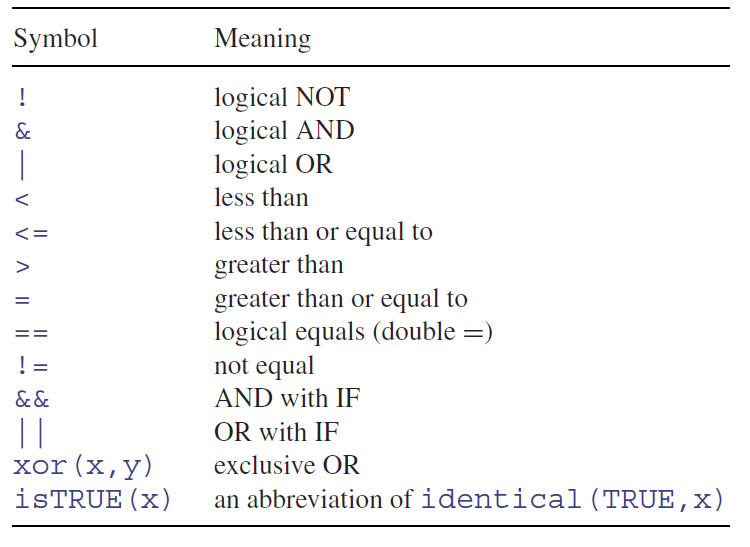
\includegraphics[scale=0.5]{logical.png}
\end{figure}
\end{center}


\end{frame}

\begin{frame}[fragile]{Booleano o de tipo Lógico (logical)}

\begin{Shaded}
\begin{Highlighting}[]
\OtherTok{TRUE} \OperatorTok{&}\StringTok{ }\OtherTok{FALSE}
\end{Highlighting}
\end{Shaded}

\begin{verbatim}
## [1] FALSE
\end{verbatim}

\begin{Shaded}
\begin{Highlighting}[]
\OtherTok{FALSE} \OperatorTok{|}\StringTok{ }\OtherTok{FALSE}
\end{Highlighting}
\end{Shaded}

\begin{verbatim}
## [1] FALSE
\end{verbatim}

\begin{Shaded}
\begin{Highlighting}[]
\OperatorTok{!}\OtherTok{TRUE}
\end{Highlighting}
\end{Shaded}

\begin{verbatim}
## [1] FALSE
\end{verbatim}

\end{frame}

\begin{frame}[fragile]{Missing Data (NA)}

Un valor faltante o valor indefinido es indicado por la instrucción NA
(por no-disponible), varias funciones existen para manejar este tipo de
dtos. De hecho, R lo considera como un valor lógico constante

\begin{Shaded}
\begin{Highlighting}[]
\NormalTok{x <-}\StringTok{ }\KeywordTok{c}\NormalTok{(}\DecValTok{3}\NormalTok{,}\OtherTok{NA}\NormalTok{,}\DecValTok{6}\NormalTok{)}
\KeywordTok{is.na}\NormalTok{(x)}
\end{Highlighting}
\end{Shaded}

\begin{verbatim}
## [1] FALSE  TRUE FALSE
\end{verbatim}

\begin{Shaded}
\begin{Highlighting}[]
\KeywordTok{mean}\NormalTok{(x)}
\end{Highlighting}
\end{Shaded}

\begin{verbatim}
## [1] NA
\end{verbatim}

\end{frame}

\begin{frame}[fragile]{Missing Data (NA)}

\begin{Shaded}
\begin{Highlighting}[]
\KeywordTok{mean}\NormalTok{(x,}\DataTypeTok{na.rm =} \OtherTok{TRUE}\NormalTok{)}
\end{Highlighting}
\end{Shaded}

\begin{verbatim}
## [1] 4.5
\end{verbatim}

Los Missing Values son una fuente de irritación, porque ellos afectan
las funciones que ajustan modelos y pueden reducir el poder del
modelamiento

\end{frame}

\begin{frame}[fragile]{Infinitos y cosas que no son números}

Los cálculos pueden conducir a respuestas como más infinito ó menos
infinito

\begin{Shaded}
\begin{Highlighting}[]
\DecValTok{3}\OperatorTok{/}\DecValTok{0}
\end{Highlighting}
\end{Shaded}

\begin{verbatim}
## [1] Inf
\end{verbatim}

\begin{Shaded}
\begin{Highlighting}[]
\OperatorTok{-}\DecValTok{12}\OperatorTok{/}\DecValTok{0}
\end{Highlighting}
\end{Shaded}

\begin{verbatim}
## [1] -Inf
\end{verbatim}

\end{frame}

\begin{frame}[fragile]{Infinitos y cosas que no son números}

Podemos operar infinitos también

\begin{Shaded}
\begin{Highlighting}[]
\KeywordTok{exp}\NormalTok{(}\OperatorTok{-}\OtherTok{Inf}\NormalTok{)}
\end{Highlighting}
\end{Shaded}

\begin{verbatim}
## [1] 0
\end{verbatim}

\begin{Shaded}
\begin{Highlighting}[]
\DecValTok{0}\OperatorTok{/}\OtherTok{Inf}
\end{Highlighting}
\end{Shaded}

\begin{verbatim}
## [1] 0
\end{verbatim}

\end{frame}

\begin{frame}[fragile]{Infinitos y cosas que no son números}

Otros cálculos conducen a cantidades que no son números

\begin{Shaded}
\begin{Highlighting}[]
\DecValTok{0}\OperatorTok{/}\DecValTok{0}
\end{Highlighting}
\end{Shaded}

\begin{verbatim}
## [1] NaN
\end{verbatim}

\begin{Shaded}
\begin{Highlighting}[]
\OtherTok{Inf}\OperatorTok{-}\OtherTok{Inf}
\end{Highlighting}
\end{Shaded}

\begin{verbatim}
## [1] NaN
\end{verbatim}

\begin{Shaded}
\begin{Highlighting}[]
\OtherTok{Inf}\OperatorTok{/}\OtherTok{Inf}
\end{Highlighting}
\end{Shaded}

\begin{verbatim}
## [1] NaN
\end{verbatim}

\end{frame}

\begin{frame}{Infinitos y cosas que no son números}

Es necesario entender la diferencia entre NaN y NA. NaN significa ``no
es un número'' y significa que es un resultado, pero no puede ser
representado en el computador. NA explica que el data es faltante por
razones desconocidas

NaN implica un resultado que no puede ser calculado por cualquier razón

\end{frame}

\begin{frame}[fragile]{Caracteres tipo String (character)}

Este tipo de dato corresponde a las citas que queramos realizar

\begin{Shaded}
\begin{Highlighting}[]
\NormalTok{a <-}\StringTok{ "R es mi amigo"}
\NormalTok{a}
\end{Highlighting}
\end{Shaded}

\begin{verbatim}
## [1] "R es mi amigo"
\end{verbatim}

\begin{Shaded}
\begin{Highlighting}[]
\KeywordTok{typeof}\NormalTok{(a)}
\end{Highlighting}
\end{Shaded}

\begin{verbatim}
## [1] "character"
\end{verbatim}

\begin{Shaded}
\begin{Highlighting}[]
\KeywordTok{is.character}\NormalTok{(a)}
\end{Highlighting}
\end{Shaded}

\begin{verbatim}
## [1] TRUE
\end{verbatim}

\end{frame}

\begin{frame}[fragile]{Caracteres tipo String (character)}

Podemos convertir números (numeric) a carater (character) y viceversa

\begin{Shaded}
\begin{Highlighting}[]
\KeywordTok{as.character}\NormalTok{(}\FloatTok{2.3}\NormalTok{)}
\end{Highlighting}
\end{Shaded}

\begin{verbatim}
## [1] "2.3"
\end{verbatim}

\begin{Shaded}
\begin{Highlighting}[]
\KeywordTok{as.integer}\NormalTok{(}\StringTok{"3"}\NormalTok{)}
\end{Highlighting}
\end{Shaded}

\begin{verbatim}
## [1] 3
\end{verbatim}

\begin{Shaded}
\begin{Highlighting}[]
\KeywordTok{as.integer}\NormalTok{(}\StringTok{"3.cuatro"}\NormalTok{)}
\end{Highlighting}
\end{Shaded}

\begin{verbatim}
## Warning: NAs introducidos por coerción
\end{verbatim}

\begin{verbatim}
## [1] NA
\end{verbatim}

\end{frame}

\begin{frame}[fragile]{Caracteres tipo String (character)}

También podemos generar frases de tipo string

\begin{Shaded}
\begin{Highlighting}[]
\KeywordTok{cat}\NormalTok{(}\StringTok{"Hola"}\NormalTok{,}\StringTok{"mundo"}\NormalTok{,}\StringTok{"!"}\NormalTok{)}
\end{Highlighting}
\end{Shaded}

\begin{verbatim}
## Hola mundo !
\end{verbatim}

\begin{Shaded}
\begin{Highlighting}[]
\KeywordTok{cat}\NormalTok{(}\StringTok{"Hello"}\NormalTok{,}\FloatTok{2.7}\NormalTok{,}\StringTok{"!"}\NormalTok{)}
\end{Highlighting}
\end{Shaded}

\begin{verbatim}
## Hello 2.7 !
\end{verbatim}

\begin{Shaded}
\begin{Highlighting}[]
\KeywordTok{paste}\NormalTok{(}\DecValTok{1}\OperatorTok{:}\DecValTok{12}\NormalTok{)}
\end{Highlighting}
\end{Shaded}

\begin{verbatim}
##  [1] "1"  "2"  "3"  "4"  "5"  "6"  "7"  "8"  "9" 
##[10] "10" "11" "12"
\end{verbatim}

\end{frame}

\begin{frame}[fragile]{Caracteres tipo String (character)}

\begin{Shaded}
\begin{Highlighting}[]
\KeywordTok{paste}\NormalTok{(}\StringTok{"Hola"}\NormalTok{,}\StringTok{"mundo"}\NormalTok{,}\StringTok{"!"}\NormalTok{,}\DataTypeTok{sep =} \StringTok{" "}\NormalTok{)}
\end{Highlighting}
\end{Shaded}

\begin{verbatim}
## [1] "Hola mundo !"
\end{verbatim}

\begin{Shaded}
\begin{Highlighting}[]
\KeywordTok{paste}\NormalTok{(}\StringTok{"Hola"}\NormalTok{,}\DecValTok{2}\NormalTok{,}\StringTok{"!"}\NormalTok{,}\DataTypeTok{collapse =} \StringTok{" "}\NormalTok{)}
\end{Highlighting}
\end{Shaded}

\begin{verbatim}
## [1] "Hola 2 !"
\end{verbatim}

\end{frame}

\begin{frame}{Estructuras de Datos}

En R se pueden organizar varios tipod de datos, mediante distintas
estructuras que permiten realizar diferentes acciones sobre ellas

\end{frame}

\begin{frame}[fragile]{Estructuras de Datos: Vectores (vector)}

Es la estructura de datos más simple. Representa un secuencia de datos
del mismo tipo

\begin{Shaded}
\begin{Highlighting}[]
\DecValTok{0}\OperatorTok{:}\DecValTok{10}
\end{Highlighting}
\end{Shaded}

\begin{verbatim}
##  [1]  0  1  2  3  4  5  6  7  8  9 10
\end{verbatim}

\begin{Shaded}
\begin{Highlighting}[]
\DecValTok{15}\OperatorTok{:}\DecValTok{5}
\end{Highlighting}
\end{Shaded}

\begin{verbatim}
##  [1] 15 14 13 12 11 10  9  8  7  6  5
\end{verbatim}

\begin{Shaded}
\begin{Highlighting}[]
\KeywordTok{c}\NormalTok{(}\DecValTok{55}\NormalTok{, }\DecValTok{76}\NormalTok{, }\DecValTok{92}\NormalTok{, }\DecValTok{103}\NormalTok{, }\DecValTok{84}\NormalTok{, }\DecValTok{88}\NormalTok{, }\DecValTok{121}\NormalTok{, }\DecValTok{91}\NormalTok{, }\DecValTok{65}\NormalTok{, }\DecValTok{77}\NormalTok{, }\DecValTok{99}\NormalTok{)}
\end{Highlighting}
\end{Shaded}

\begin{verbatim}
##  [1]  55  76  92 103  84  88 121  91  65  77  99
\end{verbatim}

\end{frame}

\begin{frame}[fragile]{Estructuras de Datos: Vectores (vector)}

\begin{Shaded}
\begin{Highlighting}[]
\KeywordTok{seq}\NormalTok{(}\DataTypeTok{from=}\FloatTok{0.04}\NormalTok{,}\DataTypeTok{by=}\FloatTok{0.01}\NormalTok{,}\DataTypeTok{length=}\DecValTok{11}\NormalTok{)}
\end{Highlighting}
\end{Shaded}

\begin{verbatim}
##  [1] 0.04 0.05 0.06 0.07 0.08 0.09 0.10 0.11 0.12
##  [9] 0.13 0.14
\end{verbatim}

\begin{Shaded}
\begin{Highlighting}[]
\KeywordTok{seq}\NormalTok{(}\DataTypeTok{from=}\FloatTok{0.2}\NormalTok{, }\DataTypeTok{to=}\DecValTok{4}\NormalTok{, }\DataTypeTok{by=}\FloatTok{0.2}\NormalTok{)}
\end{Highlighting}
\end{Shaded}

\begin{verbatim}
##  [1] 0.2 0.4 0.6 0.8 1.0 1.2 1.4 1.6 1.8 2.0 2.2
## [12] 2.4 2.6 2.8 3.0 3.2 3.4 3.6 3.8 4.0
\end{verbatim}

\begin{Shaded}
\begin{Highlighting}[]
\KeywordTok{seq}\NormalTok{(}\DecValTok{0}\NormalTok{, }\FloatTok{1.5}\NormalTok{, }\FloatTok{0.1}\NormalTok{)}
\end{Highlighting}
\end{Shaded}

\begin{verbatim}
##  [1] 0.0 0.1 0.2 0.3 0.4 0.5 0.6 0.7 0.8 0.9 1.0 1.1 
## [12]1.2 1.3 1.4 1.5
\end{verbatim}

\end{frame}

\begin{frame}[fragile]{Estructuras de Datos: Vectores (vector)}

\begin{Shaded}
\begin{Highlighting}[]
\KeywordTok{seq}\NormalTok{(}\DecValTok{6}\NormalTok{, }\DecValTok{4}\NormalTok{, }\OperatorTok{-}\FloatTok{0.2}\NormalTok{)}
\end{Highlighting}
\end{Shaded}

\begin{verbatim}
##  [1] 6.0 5.8 5.6 5.4 5.2 5.0 4.8 4.6 4.4 4.2 4.0
\end{verbatim}

\begin{Shaded}
\begin{Highlighting}[]
\NormalTok{N <-}\StringTok{ }\KeywordTok{c}\NormalTok{(}\DecValTok{55}\NormalTok{, }\DecValTok{76}\NormalTok{, }\DecValTok{92}\NormalTok{, }\DecValTok{103}\NormalTok{, }\DecValTok{84}\NormalTok{, }\DecValTok{88}\NormalTok{, }\DecValTok{121}\NormalTok{, }\DecValTok{91}\NormalTok{, }\DecValTok{65}\NormalTok{, }\DecValTok{77}\NormalTok{, }\DecValTok{99}\NormalTok{)}
\end{Highlighting}
\end{Shaded}

Si queremos usar el largo de N en otro vector usamos

\begin{Shaded}
\begin{Highlighting}[]
\KeywordTok{seq}\NormalTok{(}\DataTypeTok{from=}\FloatTok{0.04}\NormalTok{, }\DataTypeTok{by=}\FloatTok{0.01}\NormalTok{, }\DataTypeTok{along=}\NormalTok{N)}
\end{Highlighting}
\end{Shaded}

\begin{verbatim}
##  [1] 0.04 0.05 0.06 0.07 0.08 0.09 0.10 0.11 0.12
## [10] 0.13 0.14
\end{verbatim}

\end{frame}

\begin{frame}[fragile]{Estructuras de Datos: Vectores (vector)}

\begin{Shaded}
\begin{Highlighting}[]
\KeywordTok{seq}\NormalTok{(}\DataTypeTok{from=}\FloatTok{0.04}\NormalTok{, }\DataTypeTok{to=}\FloatTok{0.14}\NormalTok{, }\DataTypeTok{along=}\NormalTok{N)}
\end{Highlighting}
\end{Shaded}

\begin{verbatim}
##  [1] 0.04 0.05 0.06 0.07 0.08 0.09 0.10 0.11 0.12
## [10] 0.13 0.14
\end{verbatim}

Observe que cuando el incremento no coincide con el valor final,
entonces la secuencia generada para antes del último valor

\begin{Shaded}
\begin{Highlighting}[]
\KeywordTok{seq}\NormalTok{(}\FloatTok{1.4}\NormalTok{, }\FloatTok{2.1}\NormalTok{, }\FloatTok{0.3}\NormalTok{)}
\end{Highlighting}
\end{Shaded}

\begin{verbatim}
## [1] 1.4 1.7 2.0
\end{verbatim}

\end{frame}

\begin{frame}[fragile]{Estructuras de Datos: Vectores (vector)}

Si queremos generar varias sequencias de vectores con diferente tamaños
usamos

\begin{Shaded}
\begin{Highlighting}[]
\KeywordTok{sequence}\NormalTok{(}\KeywordTok{c}\NormalTok{(}\DecValTok{4}\NormalTok{,}\DecValTok{3}\NormalTok{,}\DecValTok{4}\NormalTok{,}\DecValTok{4}\NormalTok{,}\DecValTok{4}\NormalTok{,}\DecValTok{5}\NormalTok{))}
\end{Highlighting}
\end{Shaded}

\begin{verbatim}
##  [1] 1 2 3 4 1 2 3 1 2 3 4 1 2 3 4 1 2 3 4 1 2 3 4 5
\end{verbatim}

para generar reprticiones de números o caracteres usamos

\begin{Shaded}
\begin{Highlighting}[]
\KeywordTok{rep}\NormalTok{(}\DecValTok{9}\NormalTok{,}\DecValTok{5}\NormalTok{)}
\end{Highlighting}
\end{Shaded}

\begin{verbatim}
## [1] 9 9 9 9 9
\end{verbatim}

\end{frame}

\begin{frame}[fragile]{Estructuras de Datos: Vectores (vector)}

\begin{Shaded}
\begin{Highlighting}[]
\KeywordTok{rep}\NormalTok{(}\DecValTok{1}\OperatorTok{:}\DecValTok{4}\NormalTok{, }\DecValTok{2}\NormalTok{)}
\end{Highlighting}
\end{Shaded}

\begin{verbatim}
## [1] 1 2 3 4 1 2 3 4
\end{verbatim}

\begin{Shaded}
\begin{Highlighting}[]
\KeywordTok{rep}\NormalTok{(}\DecValTok{1}\OperatorTok{:}\DecValTok{4}\NormalTok{,}\DataTypeTok{each =} \DecValTok{2}\NormalTok{)}
\end{Highlighting}
\end{Shaded}

\begin{verbatim}
## [1] 1 1 2 2 3 3 4 4
\end{verbatim}

\begin{Shaded}
\begin{Highlighting}[]
\KeywordTok{rep}\NormalTok{(}\DecValTok{1}\OperatorTok{:}\DecValTok{4}\NormalTok{, }\DataTypeTok{each =} \DecValTok{2}\NormalTok{, }\DataTypeTok{times =} \DecValTok{3}\NormalTok{)}
\end{Highlighting}
\end{Shaded}

\begin{verbatim}
##  [1] 1 1 2 2 3 3 4 4 1 1 2 2 3 3 4 4 1 1 2 2 3 3 4 4
\end{verbatim}

\end{frame}

\begin{frame}[fragile]{Estructuras de Datos: Vectores (vector)}

Para repetir números pero diferente número de veces usamos un vector que
nos especifique el números de veces con respecto al ubicación del número

\begin{Shaded}
\begin{Highlighting}[]
\KeywordTok{rep}\NormalTok{(}\DecValTok{1}\OperatorTok{:}\DecValTok{4}\NormalTok{,}\DecValTok{1}\OperatorTok{:}\DecValTok{4}\NormalTok{)}
\end{Highlighting}
\end{Shaded}

\begin{verbatim}
##  [1] 1 2 2 3 3 3 4 4 4 4
\end{verbatim}

\begin{Shaded}
\begin{Highlighting}[]
\KeywordTok{rep}\NormalTok{(}\DecValTok{1}\OperatorTok{:}\DecValTok{4}\NormalTok{,}\KeywordTok{c}\NormalTok{(}\DecValTok{4}\NormalTok{,}\DecValTok{1}\NormalTok{,}\DecValTok{4}\NormalTok{,}\DecValTok{2}\NormalTok{))}
\end{Highlighting}
\end{Shaded}

\begin{verbatim}
##  [1] 1 1 1 1 2 3 3 3 3 4 4
\end{verbatim}

\end{frame}

\begin{frame}[fragile]{Estructuras de Datos: Vectores (vector)}

usándolo para caracteres

\begin{Shaded}
\begin{Highlighting}[]
\KeywordTok{rep}\NormalTok{(}\KeywordTok{c}\NormalTok{(}\StringTok{"gato"}\NormalTok{,}\StringTok{"perro"}\NormalTok{,}\StringTok{"pez"}\NormalTok{,}\StringTok{"ratón","}\NormalTok{conejo}\StringTok{")}
\StringTok{    ,c(2,3,2,1,3))}
\end{Highlighting}
\end{Shaded}

\begin{verbatim}
##  [1] "gato"   "gato"   "perro"  "perro"  "perro"  "pez"    "pez"   
##  [7] "pez"  "ratón"  "conejo" "conejo" "conejo"
\end{verbatim}

Cuando usamos la función c() establecemos un vector de datos tipo
double, sin embargo, si los datos son de tipo entero los podemos
convertir a enteros (integer), con el objetivo de consumir menor memoria

\begin{Shaded}
\begin{Highlighting}[]
\NormalTok{x <-}\StringTok{ }\KeywordTok{c}\NormalTok{(}\DecValTok{5}\NormalTok{,}\DecValTok{3}\NormalTok{,}\DecValTok{7}\NormalTok{,}\DecValTok{8}\NormalTok{)}
\end{Highlighting}
\end{Shaded}

estos vectores de datos tipo double se denominan numeric

\begin{Shaded}
\begin{Highlighting}[]
\KeywordTok{class}\NormalTok{(x)}
\end{Highlighting}
\end{Shaded}

\begin{verbatim}
## [1] "numeric"
\end{verbatim}

\end{frame}

\begin{frame}[fragile]{Estructuras de Datos: Vectores (vector)}

\begin{Shaded}
\begin{Highlighting}[]
\KeywordTok{is.numeric}\NormalTok{(x)}
\end{Highlighting}
\end{Shaded}

\begin{verbatim}
## [1] TRUE
\end{verbatim}

\begin{Shaded}
\begin{Highlighting}[]
\KeywordTok{is.integer}\NormalTok{(x)}
\end{Highlighting}
\end{Shaded}

\begin{verbatim}
## [1] FALSE
\end{verbatim}

realizando coerción

\begin{Shaded}
\begin{Highlighting}[]
\NormalTok{x <-}\StringTok{ }\KeywordTok{as.integer}\NormalTok{(x)}
\end{Highlighting}
\end{Shaded}

\end{frame}

\begin{frame}[fragile]{Estructuras de Datos: Vectores (vector)}

\begin{Shaded}
\begin{Highlighting}[]
\KeywordTok{is.integer}\NormalTok{(x)}
\end{Highlighting}
\end{Shaded}

\begin{verbatim}
## [1] TRUE
\end{verbatim}

Para ponerle nombre a los elementos de un vector procedemos

\begin{Shaded}
\begin{Highlighting}[]
\NormalTok{vec<-}\KeywordTok{c}\NormalTok{(}\DecValTok{1}\NormalTok{,}\DecValTok{3}\NormalTok{,}\DecValTok{6}\NormalTok{,}\DecValTok{2}\NormalTok{,}\DecValTok{7}\NormalTok{,}\DecValTok{4}\NormalTok{,}\DecValTok{8}\NormalTok{,}\DecValTok{1}\NormalTok{,}\DecValTok{0}\NormalTok{)}
\KeywordTok{names}\NormalTok{(vec)<-}\StringTok{ }\KeywordTok{c}\NormalTok{(}\StringTok{"aa"}\NormalTok{,}\StringTok{"bb"}\NormalTok{,}\StringTok{"cc"}\NormalTok{,}\StringTok{"dd"}\NormalTok{,}\StringTok{"ee"}\NormalTok{,}\StringTok{"ff"}\NormalTok{,}\StringTok{"gg"}
\NormalTok{               ,}\StringTok{"hh"}\NormalTok{,}\StringTok{"ii"}\NormalTok{)}
\NormalTok{vec}
\end{Highlighting}
\end{Shaded}

\begin{verbatim}
## aa bb cc dd ee ff gg hh ii 
##  1  3  6  2  7  4  8  1  0
\end{verbatim}

\end{frame}

\begin{frame}[fragile]{Matrices (matrix) y Arrays (array)}

son representaciones de estructuras de datos con dos índices para
matrices y múltiple para arrays, como los vectores, deben ser del mismo
tipo.

\begin{Shaded}
\begin{Highlighting}[]
\NormalTok{X <-}\StringTok{ }\KeywordTok{matrix}\NormalTok{(}\KeywordTok{c}\NormalTok{(}\DecValTok{1}\NormalTok{,}\DecValTok{2}\NormalTok{,}\DecValTok{0}\NormalTok{,}\DecValTok{0}\NormalTok{,}\DecValTok{1}\NormalTok{,}\DecValTok{0}\NormalTok{,}\DecValTok{0}\NormalTok{,}\DecValTok{0}\NormalTok{,}\DecValTok{1}\NormalTok{),}\DataTypeTok{nrow =} \DecValTok{3}\NormalTok{)}
\NormalTok{X}
\end{Highlighting}
\end{Shaded}

\begin{verbatim}
##      [,1] [,2] [,3]
## [1,]    1    0    0
## [2,]    2    1    0
## [3,]    0    0    1
\end{verbatim}

\begin{Shaded}
\begin{Highlighting}[]
\KeywordTok{class}\NormalTok{(X)}
\end{Highlighting}
\end{Shaded}

\begin{verbatim}
## [1] "matrix"
\end{verbatim}

\end{frame}

\begin{frame}[fragile]{Matrices (matrix) y Arrays (array)}

\begin{Shaded}
\begin{Highlighting}[]
\KeywordTok{attributes}\NormalTok{(X)}
\end{Highlighting}
\end{Shaded}

\begin{verbatim}
## $dim
## [1] 3 3
\end{verbatim}

\begin{Shaded}
\begin{Highlighting}[]
\NormalTok{vector <-}\StringTok{ }\KeywordTok{c}\NormalTok{(}\DecValTok{1}\NormalTok{,}\DecValTok{2}\NormalTok{,}\DecValTok{3}\NormalTok{,}\DecValTok{4}\NormalTok{,}\DecValTok{4}\NormalTok{,}\DecValTok{3}\NormalTok{,}\DecValTok{2}\NormalTok{,}\DecValTok{1}\NormalTok{)}
\NormalTok{V <-}\StringTok{ }\KeywordTok{matrix}\NormalTok{(vector,}\DataTypeTok{byrow =}\NormalTok{ T,}\DataTypeTok{nrow =} \DecValTok{2}\NormalTok{)}
\NormalTok{V}
\end{Highlighting}
\end{Shaded}

\begin{verbatim}
##      [,1] [,2] [,3] [,4]
## [1,]    1    3    4    2
## [2,]    2    4    3    1
\end{verbatim}

otra forma de convertir un vector a matrix es con

\begin{Shaded}
\begin{Highlighting}[]
\KeywordTok{dim}\NormalTok{(vector) <-}\StringTok{ }\KeywordTok{c}\NormalTok{(}\DecValTok{4}\NormalTok{,}\DecValTok{2}\NormalTok{)}
\end{Highlighting}
\end{Shaded}

\end{frame}

\begin{frame}[fragile]{Matrices (matrix) y Arrays (array)}

\begin{Shaded}
\begin{Highlighting}[]
\KeywordTok{is.matrix}\NormalTok{(vector)}
\end{Highlighting}
\end{Shaded}

\begin{verbatim}
## [1] TRUE
\end{verbatim}

\begin{Shaded}
\begin{Highlighting}[]
\NormalTok{vector}
\end{Highlighting}
\end{Shaded}

\begin{verbatim}
##      [,1] [,2]
## [1,]    1    4
## [2,]    2    3
## [3,]    3    2
## [4,]    4    1
\end{verbatim}

\end{frame}

\begin{frame}[fragile]{Matrices (matrix) y Arrays (array)}

\begin{Shaded}
\begin{Highlighting}[]
\NormalTok{vector <-}\StringTok{ }\KeywordTok{t}\NormalTok{(vector)}
\NormalTok{vector}
\end{Highlighting}
\end{Shaded}

\begin{verbatim}
##      [,1] [,2] [,3] [,4]
## [1,]    1    2    3    4
## [2,]    4    3    2    1
\end{verbatim}

\begin{Shaded}
\begin{Highlighting}[]
\NormalTok{Y <-}\StringTok{ }\KeywordTok{matrix}\NormalTok{(}\DecValTok{1}\OperatorTok{:}\DecValTok{12}\NormalTok{,}\DataTypeTok{nrow =} \DecValTok{4}\NormalTok{,}\DataTypeTok{ncol =} \DecValTok{3}\NormalTok{,}\DataTypeTok{byrow =} \OtherTok{TRUE}\NormalTok{)}
\NormalTok{Y}
\end{Highlighting}
\end{Shaded}

\begin{verbatim}
##      [,1] [,2] [,3]
## [1,]    1    2    3
## [2,]    4    5    6
## [3,]    7    8    9
## [4,]   10   11   12
\end{verbatim}

\end{frame}

\begin{frame}[fragile]{Matrices (matrix) y Arrays (array)}

Para colocar nombres a nuestras filas y columnas en una matriz usamos

\begin{Shaded}
\begin{Highlighting}[]
\NormalTok{X <-}\StringTok{ }\KeywordTok{matrix}\NormalTok{(}\KeywordTok{rpois}\NormalTok{(}\DecValTok{20}\NormalTok{,}\FloatTok{1.5}\NormalTok{),}\DataTypeTok{nrow=}\DecValTok{4}\NormalTok{)}
\NormalTok{X}
\end{Highlighting}
\end{Shaded}

\begin{verbatim}
##      [,1] [,2] [,3] [,4] [,5]
## [1,]    4    2    2    1    3
## [2,]    2    0    0    4    4
## [3,]    2    0    0    1    1
## [4,]    2    3    2    2    1
\end{verbatim}

\end{frame}

\begin{frame}[fragile]{Matrices (matrix) y Arrays (array)}

donde do.NULL = FALSE nos da los números y el prefix el prefijo

\begin{Shaded}
\begin{Highlighting}[]
\KeywordTok{rownames}\NormalTok{(X) <-}\StringTok{ }\KeywordTok{rownames}\NormalTok{(X,}\DataTypeTok{do.NULL=}\OtherTok{FALSE}\NormalTok{,}\DataTypeTok{prefix=}\StringTok{"Trial."}\NormalTok{)}
\NormalTok{X}
\end{Highlighting}
\end{Shaded}

\begin{verbatim}
##         [,1] [,2] [,3] [,4] [,5]
## Trial.1    4    2    2    1    3
## Trial.2    2    0    0    4    4
## Trial.3    2    0    0    1    1
## Trial.4    2    3    2    2    1
\end{verbatim}

\end{frame}

\begin{frame}[fragile]{Matrices (matrix) y Arrays (array)}

\begin{Shaded}
\begin{Highlighting}[]
\NormalTok{drug.names <-}\StringTok{ }\KeywordTok{c}\NormalTok{(}\StringTok{"aspirin"}\NormalTok{, }\StringTok{"paracetamol"}\NormalTok{, }\StringTok{"nurofen"}\NormalTok{,}
                \StringTok{"hedex"}\NormalTok{, }\StringTok{"placebo"}\NormalTok{)}
\KeywordTok{colnames}\NormalTok{(X) <-}\StringTok{ }\NormalTok{drug.names}
\NormalTok{X}
\end{Highlighting}
\end{Shaded}

\begin{verbatim}
##         aspirin paracetamol nurofen hedex placebo
## Trial.1       4           2       2     1       3
## Trial.2       2           0       0     4       4
## Trial.3       2           0       0     1       1
## Trial.4       2           3       2     2       1
\end{verbatim}

\end{frame}

\begin{frame}[fragile]{Matrices (matrix) y Arrays (array)}

de forma alternativa

\begin{Shaded}
\begin{Highlighting}[]
\KeywordTok{dimnames}\NormalTok{(X) <-}\StringTok{ }\KeywordTok{list}\NormalTok{(}\OtherTok{NULL}\NormalTok{,}\KeywordTok{paste}\NormalTok{(}\StringTok{"drug."}\NormalTok{,}\DecValTok{1}\OperatorTok{:}\DecValTok{5}\NormalTok{,}\DataTypeTok{sep=}\StringTok{""}\NormalTok{))}
\NormalTok{X}
\end{Highlighting}
\end{Shaded}

\begin{verbatim}
##      drug.1 drug.2 drug.3 drug.4 drug.5
## [1,]      4      2      2      1      3
## [2,]      2      0      0      4      4
## [3,]      2      0      0      1      1
## [4,]      2      3      2      2      1
\end{verbatim}

\end{frame}

\begin{frame}{Matrices (matrix) y Arrays (array)}

Los arrays corresponden a matrices multidiensionales, veamos un ejemplo
de 3 dimensiones

\begin{center}
\begin{figure}
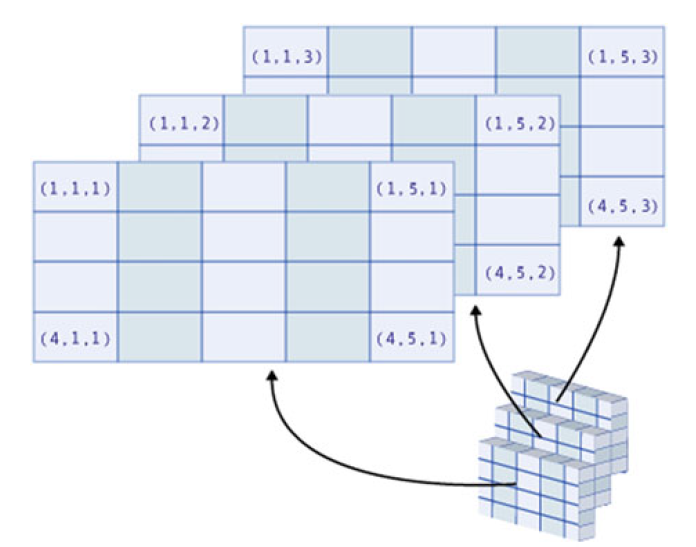
\includegraphics[scale=0.4]{array.png}
\end{figure}
\end{center}

\end{frame}

\begin{frame}[fragile]{Matrices (matrix) y Arrays (array)}

\begin{Shaded}
\begin{Highlighting}[]
\NormalTok{P <-}\StringTok{ }\KeywordTok{array}\NormalTok{(}\KeywordTok{as.integer}\NormalTok{(}\KeywordTok{rnorm}\NormalTok{(}\DecValTok{60}\NormalTok{)),}\DataTypeTok{dim =} \KeywordTok{c}\NormalTok{(}\DecValTok{4}\NormalTok{,}\DecValTok{5}\NormalTok{,}\DecValTok{3}\NormalTok{))}
\NormalTok{P}
\end{Highlighting}
\end{Shaded}

\begin{verbatim}
## , , 1
## 
##      [,1] [,2] [,3] [,4] [,5]
## [1,]    1    0    1    0    0
## [2,]    0   -2    0   -1    0
## [3,]    0    0    0    0    0
## [4,]    0    0    0    0    0
## 
\end{verbatim}

\end{frame}

\begin{frame}[fragile]{Matrices (matrix) y Arrays (array)}

\begin{verbatim}
## , , 2
## 
##      [,1] [,2] [,3] [,4] [,5]
## [1,]    0    0    0    1    0
## [2,]    0    0    0    0    0
## [3,]    0    0    0    1    0
## [4,]    0   -1    1    0    0
## 
\end{verbatim}

\end{frame}

\begin{frame}[fragile]{Matrices (matrix) y Arrays (array)}

\begin{verbatim}
## , , 3
## 
##      [,1] [,2] [,3] [,4] [,5]
## [1,]    0    0   -1   -1    0
## [2,]   -1    0    0    1    0
## [3,]    0    0    0   -1    0
## [4,]   -1    0    0    1    0
\end{verbatim}

\end{frame}

\begin{frame}[fragile]{Matrices (matrix) y Arrays (array)}

\begin{Shaded}
\begin{Highlighting}[]
\KeywordTok{class}\NormalTok{(P)}
\end{Highlighting}
\end{Shaded}

\begin{verbatim}
## [1] "array"
\end{verbatim}

\end{frame}

\begin{frame}{Listas (list)}

Son estrucutras de datos extremadamente importantes en R debido a su
riqueza y a la capacidad de agrupar en una estructura datos de diferente
tipos sin alterarlos, es decir, cada elemento de una lista puede ser un
dato, vector, matrix, array o incluso otra lista

\end{frame}

\begin{frame}[fragile]{Listas (list)}

\begin{Shaded}
\begin{Highlighting}[]
\NormalTok{A <-}\StringTok{ }\KeywordTok{list}\NormalTok{(}\OtherTok{TRUE}\NormalTok{,}\OperatorTok{-}\DecValTok{1}\OperatorTok{:}\DecValTok{3}\NormalTok{,}\KeywordTok{matrix}\NormalTok{(}\DecValTok{1}\OperatorTok{:}\DecValTok{4}\NormalTok{,}\DataTypeTok{nrow =} \DecValTok{2}\NormalTok{), }\KeywordTok{c}\NormalTok{(}\DecValTok{1}\OperatorTok{+}\NormalTok{2i,}\DecValTok{3}\NormalTok{),}
          \StringTok{"A es un character"}\NormalTok{)}
\NormalTok{A}
\end{Highlighting}
\end{Shaded}

\begin{verbatim}
## [[1]]
## [1] TRUE
## 
## [[2]]
## [1] -1  0  1  2  3
## 
## [[3]]
##      [,1] [,2]
## [1,]    1    3
## [2,]    2    4
## 
\end{verbatim}

\end{frame}

\begin{frame}[fragile]{Listas (list)}

\begin{verbatim}
## [[4]]
## [1] 1+2i 3+0i
## 
## [[5]]
## [1] "A es un character"
\end{verbatim}

\end{frame}

\begin{frame}[fragile]{Listas (list)}

\begin{Shaded}
\begin{Highlighting}[]
\KeywordTok{class}\NormalTok{(A)}
\end{Highlighting}
\end{Shaded}

\begin{verbatim}
## [1] "list"
\end{verbatim}

\begin{Shaded}
\begin{Highlighting}[]
\NormalTok{apples <-}\StringTok{ }\KeywordTok{c}\NormalTok{(}\DecValTok{4}\NormalTok{,}\FloatTok{4.5}\NormalTok{,}\FloatTok{4.2}\NormalTok{,}\FloatTok{5.1}\NormalTok{,}\FloatTok{3.9}\NormalTok{)}
\NormalTok{orange <-}\StringTok{ }\KeywordTok{c}\NormalTok{(}\OtherTok{TRUE}\NormalTok{, }\OtherTok{TRUE}\NormalTok{, }\OtherTok{FALSE}\NormalTok{)}
\NormalTok{chalk <-}\StringTok{ }\KeywordTok{c}\NormalTok{(}\StringTok{"limestone"}\NormalTok{, }\StringTok{"marl"}\NormalTok{, }\StringTok{"oolite"}\NormalTok{, }\StringTok{"CaC03"}\NormalTok{)}
\NormalTok{cheese <-}\StringTok{ }\KeywordTok{c}\NormalTok{(}\FloatTok{3.2}\OperatorTok{-}\FloatTok{4.}\NormalTok{5i,}\FloatTok{12.8}\OperatorTok{+}\FloatTok{2.}\NormalTok{2i)}
\end{Highlighting}
\end{Shaded}

\end{frame}

\begin{frame}[fragile]{Listas (list)}

\begin{Shaded}
\begin{Highlighting}[]
\NormalTok{items <-}\StringTok{ }\KeywordTok{list}\NormalTok{(apples,orange,chalk,cheese)}
\NormalTok{items}
\end{Highlighting}
\end{Shaded}

\begin{verbatim}
## [[1]]
## [1] 4.0 4.5 4.2 5.1 3.9
## 
## [[2]]
## [1]  TRUE  TRUE FALSE
## 
## [[3]]
## [1] "limestone" "marl"      "oolite"    "CaC03"    
## 
## [[4]]
## [1]  3.2-4.5i 12.8+2.2i
\end{verbatim}

\end{frame}

\begin{frame}[fragile]{Listas (list)}

Si quiero ponerle nombre a cada elemento de la lista

\begin{Shaded}
\begin{Highlighting}[]
\NormalTok{items <-}\StringTok{ }\KeywordTok{list}\NormalTok{(}\DataTypeTok{first=}\NormalTok{apples,}\DataTypeTok{second=}\NormalTok{orange,}\DataTypeTok{third=}\NormalTok{chalk,}
              \DataTypeTok{fourth=}\NormalTok{cheese)}
\NormalTok{items}
\end{Highlighting}
\end{Shaded}

\begin{verbatim}
## $first
## [1] 4.0 4.5 4.2 5.1 3.9
## 
## $second
## [1]  TRUE  TRUE FALSE
## 
## $third
## [1] "limestone" "marl"      "oolite"    "CaC03"    
## 
## $fourth
## [1]  3.2-4.5i 12.8+2.2i
\end{verbatim}

\end{frame}

\begin{frame}[fragile]{Listas (list)}

\begin{Shaded}
\begin{Highlighting}[]
\KeywordTok{names}\NormalTok{(items)}
\end{Highlighting}
\end{Shaded}

\begin{verbatim}
## [1] "first"  "second" "third"  "fourth"
\end{verbatim}

\begin{Shaded}
\begin{Highlighting}[]
\KeywordTok{is.list}\NormalTok{(items)}
\end{Highlighting}
\end{Shaded}

\begin{verbatim}
## [1] TRUE
\end{verbatim}

\end{frame}

\begin{frame}[fragile]{Factores (factor) y variables ordinales
(ordered)}

Los factores son una estructura de variables categóricas que tienen un
número fijo de niveles, un simple ejemplo de variables categóricas puede
ser hobre o mujer

\begin{Shaded}
\begin{Highlighting}[]
\NormalTok{genero <-}\StringTok{ }\KeywordTok{factor}\NormalTok{(}\KeywordTok{c}\NormalTok{(}\StringTok{"mujer"}\NormalTok{, }\StringTok{"hombre"}\NormalTok{, }\StringTok{"mujer"}
\NormalTok{                   , }\StringTok{"hombre"}\NormalTok{, }\StringTok{"mujer"}\NormalTok{))}
\NormalTok{genero}
\end{Highlighting}
\end{Shaded}

\begin{verbatim}
## [1] mujer  hombre mujer  hombre mujer 
## Levels: hombre mujer
\end{verbatim}

\begin{Shaded}
\begin{Highlighting}[]
\KeywordTok{levels}\NormalTok{(genero)}
\end{Highlighting}
\end{Shaded}

\begin{verbatim}
## [1] "hombre" "mujer"
\end{verbatim}

\end{frame}

\begin{frame}[fragile]{Factores (factor) y variables ordinales
(ordered)}

\begin{Shaded}
\begin{Highlighting}[]
\KeywordTok{class}\NormalTok{(genero)}
\end{Highlighting}
\end{Shaded}

\begin{verbatim}
## [1] "factor"
\end{verbatim}

podemos establecer factores con número que ellos establezcan una
caraterística

\begin{Shaded}
\begin{Highlighting}[]
\NormalTok{Temp <-}\StringTok{ }\KeywordTok{factor}\NormalTok{(}\KeywordTok{c}\NormalTok{(}\DecValTok{0}\NormalTok{,}\DecValTok{1}\NormalTok{,}\DecValTok{0}\NormalTok{,}\DecValTok{3}\NormalTok{,}\DecValTok{1}\NormalTok{,}\DecValTok{0}\NormalTok{,}\DecValTok{1}\NormalTok{,}\DecValTok{0}\NormalTok{,}\DecValTok{3}\NormalTok{,}\DecValTok{3}\NormalTok{), }
               \DataTypeTok{labels =} \KeywordTok{c}\NormalTok{(}\StringTok{"Low"}\NormalTok{,}\StringTok{"medium"}\NormalTok{, }\StringTok{"High"}\NormalTok{))}
\NormalTok{Temp}
\end{Highlighting}
\end{Shaded}

\begin{verbatim}
##  [1] Low  medium  Low  High  medium  Low
##  [7] medium  Low  High High  
## Levels: Low medium High
\end{verbatim}

\end{frame}

\begin{frame}[fragile]{Factores (factor) y variables ordinales
(ordered)}

La función gl permite generar niveles y es útil para cuando se quieren
codificar grandes vectores de niveles de factor, los argumentos dice n:
hasta donde, k: cuantas veces se repite, labels: que niveles quiero

\begin{Shaded}
\begin{Highlighting}[]
\NormalTok{Imp <-}\StringTok{ }\KeywordTok{gl}\NormalTok{(}\DataTypeTok{n =} \DecValTok{2}\NormalTok{,}\DataTypeTok{k =} \DecValTok{8}\NormalTok{,}\DataTypeTok{labels =} \KeywordTok{c}\NormalTok{(}\StringTok{"Control"}\NormalTok{, }\StringTok{"Treat"}\NormalTok{))}
\NormalTok{Imp}
\end{Highlighting}
\end{Shaded}

\begin{verbatim}
##  [1] Control Control Control Control Control Control 
##  [7] Control Control Treat   Treat   Treat   Treat  
## [13] Treat   Treat   Treat   Treat  
## Levels: Control Treat
\end{verbatim}

\end{frame}

\begin{frame}[fragile]{Factores (factor) y variables ordinales
(ordered)}

\begin{Shaded}
\begin{Highlighting}[]
\KeywordTok{gl}\NormalTok{(}\DecValTok{4}\NormalTok{,}\DecValTok{3}\NormalTok{,}\DecValTok{24}\NormalTok{)}
\end{Highlighting}
\end{Shaded}

\begin{verbatim}
##  [1] 1 1 1 2 2 2 3 3 3 4 4 4 1 1 1 2 2 2 3 3 3 4 4 4
## Levels: 1 2 3 4
\end{verbatim}

Los elementos de tipo ordered tratan cuanto tenemos jerarquía en
nuestras variables cualitativas

\end{frame}

\begin{frame}[fragile]{Factores (factor) y variables ordinales
(ordered)}

\begin{Shaded}
\begin{Highlighting}[]
\NormalTok{z <-}\StringTok{ }\KeywordTok{ordered}\NormalTok{(}\KeywordTok{c}\NormalTok{(}\StringTok{"Small"}\NormalTok{,}\StringTok{"Tall"}\NormalTok{,}\StringTok{"Average"}\NormalTok{,}\StringTok{"Tall"}\NormalTok{,}
               \StringTok{"Average"}\NormalTok{,}\StringTok{"Small"}\NormalTok{,}\StringTok{"Small"}\NormalTok{),}
             \DataTypeTok{levels=}\KeywordTok{c}\NormalTok{(}\StringTok{"Small"}\NormalTok{,}\StringTok{"Average"}\NormalTok{,}\StringTok{"Tall"}\NormalTok{))}
\NormalTok{z}
\end{Highlighting}
\end{Shaded}

\begin{verbatim}
## [1] Small  Tall  Average  Tal  Average 
## [6] Small   Small  
## Levels: Small < Average < Tall
\end{verbatim}

\begin{Shaded}
\begin{Highlighting}[]
\KeywordTok{class}\NormalTok{(z)}
\end{Highlighting}
\end{Shaded}

\begin{verbatim}
## [1] "ordered" "factor"
\end{verbatim}

\end{frame}

\begin{frame}[fragile]{Unidades de tiempo (date)}

Son las unidades que conciernen a horarios, para desplegar la hora
actual

\begin{Shaded}
\begin{Highlighting}[]
\KeywordTok{Sys.time}\NormalTok{()}
\end{Highlighting}
\end{Shaded}

\begin{verbatim}
## [1] "2020-02-14 01:06:14 -05"
\end{verbatim}

\begin{Shaded}
\begin{Highlighting}[]
\KeywordTok{date}\NormalTok{()}
\end{Highlighting}
\end{Shaded}

\begin{verbatim}
## [1] "Fri Feb 14 01:06:14 2020"
\end{verbatim}

\end{frame}

\begin{frame}[fragile]{Unidades de tiempo (date)}

Realizando un vector de fechas, tenemos que

\begin{Shaded}
\begin{Highlighting}[]
\NormalTok{fechas <-}\StringTok{ }\KeywordTok{c}\NormalTok{(}\StringTok{"92/27/02"}\NormalTok{, }\StringTok{"92/02/27"}\NormalTok{, }\StringTok{"92/01/14"}\NormalTok{, }
            \StringTok{"92/02/28"}\NormalTok{, }\StringTok{"92/02/01"}\NormalTok{)}
\NormalTok{fechas <-}\StringTok{ }\KeywordTok{as.Date}\NormalTok{(fechas, }\StringTok{"%y/%m/%d"}\NormalTok{)}
\NormalTok{fechas}
\end{Highlighting}
\end{Shaded}

\begin{verbatim}
## [1] NA "1992-02-27" "1992-01-14" "1992-02-28" 
## [5] "1992-02-01"
\end{verbatim}

\begin{Shaded}
\begin{Highlighting}[]
\KeywordTok{class}\NormalTok{(fechas)}
\end{Highlighting}
\end{Shaded}

\begin{verbatim}
## [1] "Date"
\end{verbatim}

\end{frame}

\begin{frame}[fragile]{Series de tiempo (ts)}

Los datos correspondientes a Series de tiempo se establecen con la
función ts()

\begin{Shaded}
\begin{Highlighting}[]
\NormalTok{ti <-}\StringTok{ }\KeywordTok{ts}\NormalTok{(}\DecValTok{1}\OperatorTok{:}\DecValTok{10}\NormalTok{, }\DataTypeTok{frequency =} \DecValTok{12}\NormalTok{, }\DataTypeTok{start =} \KeywordTok{c}\NormalTok{(}\DecValTok{1959}\NormalTok{, }\DecValTok{2}\NormalTok{))}
\NormalTok{ti}
\end{Highlighting}
\end{Shaded}

\begin{verbatim}
##      Feb Mar Apr May Jun Jul Aug Sep Oct Nov
## 1959   1   2   3   4   5   6   7   8   9  10
\end{verbatim}

\begin{Shaded}
\begin{Highlighting}[]
\KeywordTok{ts}\NormalTok{(}\DecValTok{1}\OperatorTok{:}\DecValTok{10}\NormalTok{, }\DataTypeTok{frequency =} \DecValTok{4}\NormalTok{, }\DataTypeTok{start =} \KeywordTok{c}\NormalTok{(}\DecValTok{1959}\NormalTok{, }\DecValTok{2}\NormalTok{))}
\end{Highlighting}
\end{Shaded}

\begin{verbatim}
##      Qtr1 Qtr2 Qtr3 Qtr4
## 1959         1    2    3
## 1960    4    5    6    7
## 1961    8    9   10
\end{verbatim}

\end{frame}

\begin{frame}[fragile]{Series de tiempo (ts)}

\begin{Shaded}
\begin{Highlighting}[]
\NormalTok{ti2 <-}\StringTok{ }\KeywordTok{ts}\NormalTok{(}\DecValTok{1}\OperatorTok{:}\DecValTok{10}\NormalTok{, }\DataTypeTok{frequency =}\DecValTok{1}\OperatorTok{/}\DecValTok{12}\NormalTok{ , }\DataTypeTok{start =} \KeywordTok{c}\NormalTok{(}\DecValTok{1959}\NormalTok{))}
\NormalTok{ti2}
\end{Highlighting}
\end{Shaded}

\begin{verbatim}
## Time Series:
## Start = 1959 
## End = 2067 
## Frequency = 0.0833333333333333 
##  [1]  1  2  3  4  5  6  7  8  9 10
\end{verbatim}

\begin{Shaded}
\begin{Highlighting}[]
\KeywordTok{attributes}\NormalTok{(ti)}
\end{Highlighting}
\end{Shaded}

\begin{verbatim}
## $tsp
## [1] 1959.083 1959.833   12.000
## 
## $class
## [1] "ts"
\end{verbatim}

\end{frame}

\begin{frame}[fragile]{data frame (data.frame)}

Es una tbla de individuo X variable que es esencial en el análisis
estadísticos

\begin{Shaded}
\begin{Highlighting}[]
\NormalTok{datos <-}\StringTok{ }\KeywordTok{data.frame}\NormalTok{(}\DataTypeTok{Genero=}\KeywordTok{c}\NormalTok{(}\StringTok{"M"}\NormalTok{,}\StringTok{"F"}\NormalTok{,}\StringTok{"M"}\NormalTok{,}\StringTok{"F"}\NormalTok{,}\StringTok{" "}\NormalTok{,}\StringTok{"F"}\NormalTok{),}
                    \DataTypeTok{Altura=}\KeywordTok{c}\NormalTok{(}\FloatTok{1.83}\NormalTok{,}\FloatTok{1.76}\NormalTok{,}\FloatTok{1.82}\NormalTok{,}\FloatTok{1.60}\NormalTok{,}\FloatTok{1.90}\NormalTok{,}
                             \FloatTok{1.66}\NormalTok{),}
                    \DataTypeTok{Peso=}\KeywordTok{c}\NormalTok{(}\DecValTok{67}\NormalTok{,}\DecValTok{58}\NormalTok{,}\DecValTok{66}\NormalTok{,}\DecValTok{48}\NormalTok{,}\DecValTok{75}\NormalTok{,}\DecValTok{55}\NormalTok{),}
                    \DataTypeTok{row.names=}\KeywordTok{c}\NormalTok{(}\StringTok{"Jorge"}\NormalTok{,}\StringTok{"Julia"}\NormalTok{,}
                                \StringTok{"Henry"}\NormalTok{,}\StringTok{"Emilia"}\NormalTok{,}
                                \StringTok{"William"}\NormalTok{,}\StringTok{"Elisa"}\NormalTok{))}
\NormalTok{datos}
\end{Highlighting}
\end{Shaded}

\end{frame}

\begin{frame}[fragile]{data frame (data.frame)}

\begin{verbatim}
##         Genero Altura Peso
## Jorge        M   1.83   67
## Julia        F   1.76   58
## Henry        M   1.82   66
## Emilia       F   1.60   48
## William          1.90   75
## Elisa        F   1.66   55
\end{verbatim}

\end{frame}

\begin{frame}[fragile]{data frame (data.frame)}

\begin{Shaded}
\begin{Highlighting}[]
\KeywordTok{is.data.frame}\NormalTok{(datos)}
\end{Highlighting}
\end{Shaded}

\begin{verbatim}
## [1] TRUE
\end{verbatim}

\begin{Shaded}
\begin{Highlighting}[]
\KeywordTok{class}\NormalTok{(datos)}
\end{Highlighting}
\end{Shaded}

\begin{verbatim}
## [1] "data.frame"
\end{verbatim}

\begin{Shaded}
\begin{Highlighting}[]
\KeywordTok{str}\NormalTok{(datos)}
\end{Highlighting}
\end{Shaded}

\begin{verbatim}
## 'data.frame':    6 obs. of  3 variables:
##  $ Genero: Factor w/ 3 levels " ","F","M": 3 2 3 2 1 2
##  $ Altura: num  1.83 1.76 1.82 1.6 1.9 1.66
##  $ Peso  : num  67 58 66 48 75 55
\end{verbatim}

\end{frame}

\begin{frame}[fragile]{data frame (data.frame)}

\begin{Shaded}
\begin{Highlighting}[]
\KeywordTok{attributes}\NormalTok{(datos)}
\end{Highlighting}
\end{Shaded}

\begin{verbatim}
## $names
## [1] "Genero" "Altura" "Peso"  
## 
## $class
## [1] "data.frame"
## 
## $row.names
## [1] "Jorge"   "Julia"   "Henry"   "Emilia"  "William"
## [6] "Elisa"
\end{verbatim}

así un data frame puede ser visto como una lista cuyos elemntos tienen
igual longitud, realmente, esta es la forma como R los almacena

\end{frame}

\begin{frame}{Tabla adicional}

\begin{center}
\begin{figure}
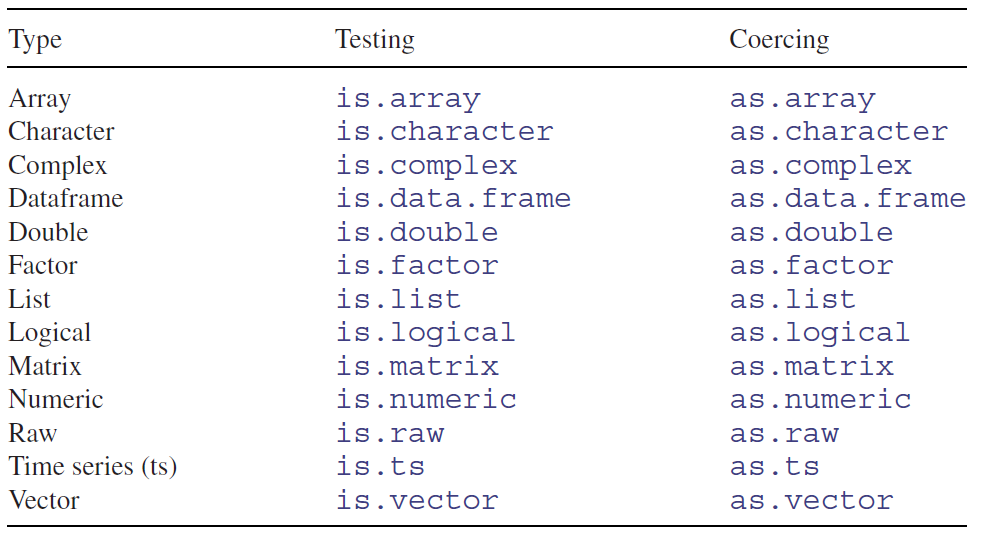
\includegraphics[scale=0.44]{coercion.png}
\end{figure}
\end{center}

\end{frame}

\end{document}
